\documentclass[
12pt, % 字体大小
a4paper, 
oneside, % 单面打印(双面为twoside)
headinclude,footinclude, % 页眉页脚包含在文本区域内,确保不被裁剪或掩盖
]{scrartcl}
% 主题和样式
\usepackage[
nochapters, % 无章节层级 
beramono, % 等宽字体样式
eulermath, % 数学公式Euler字体
pdfspacing, % 字间距
dottedtoc % 点线式目录
]{classicthesis}
\usepackage{arsclassica} 
%----------------------------------------------------------------------------------------
% 输入和页面排版
\usepackage[T1]{fontenc} % 字体编码
\usepackage[utf8]{inputenc} % 输入编码
\usepackage{ctex} % 汉语
\usepackage{amsmath,amssymb,amsthm} % 数学公式
\usepackage{indentfirst} % 缩进
\setlength{\parindent}{2em} % 段落缩进
\usepackage[
top=2cm,
bottom=2cm, 
left=2cm,
right=2cm, 
headheight=20pt, 
includeheadfoot 
]{geometry} % 页面
\usepackage{scrlayer-scrpage} % 页眉页脚
\renewcommand{\sectionmark}[1]{\markright{\spacedlowsmallcaps{#1}}}
\renewcommand{\subsectionmark}[1]{\markright{\thesubsection~#1}}
\lehead{\mbox{\llap{\small\thepage\kern1em\color{halfgray} \vline}\color{halfgray}\hspace{0.5em}\rightmark\hfil}} % 标题旁边标记页码
\cfoot{\hyperlink{toc}{\color{RoyalBlue}返回目录}} % 页脚返回目录链接
\pagestyle{scrheadings}
%----------------------------------------------------------------------------------------
% 图表和引用
\usepackage{graphicx} % 图像
\graphicspath{{Figures/}} % 图像路径
\usepackage{subfig} % 图组
\usepackage{float} % 浮动
\usepackage{enumitem} % 列表
\usepackage{varioref} % 交叉引用
%----------------------------------------------------------------------------------------
% 代码
\usepackage{listings}
\lstset{
    language=Matlab,
    basicstyle=\ttfamily\small,   % 字体
    numbers=left,                 % 行号
    numberstyle=\tiny\color{gray},
    stepnumber=5,
    numbersep=5pt,
    backgroundcolor=\color{white},% 背景
    tabsize=2,                    % 制表符宽度
    frame=single,                 % 边框
    captionpos=t,                 % 标题
    title=\lstname,
    breaklines=true,              % 换行
    breakatwhitespace=true,
    escapeinside={`}{`},          % 转义(中文注释)
}
\lstset{
    language=Python,            
    basicstyle=\ttfamily\small,   % 字体
    numbers=left,                 % 行号
    numberstyle=\tiny\color{gray}, 
    stepnumber=5,             
    numbersep=5pt,            
    backgroundcolor=\color{white},% 背景
    tabsize=4,                    % 制表符宽度            
    frame=single,                 % 边框
    captionpos=t,                 % 标题
    title=\lstname, 
    breaklines=true,              % 换行
    breakatwhitespace=false,   
    escapeinside={`}{`},          % 转义(中文注释)
}
\usepackage{algorithm} % 算法
\usepackage{algpseudocode}
\usepackage{mdframed} % 跨页框架
% 不浮动算法环境
\newcounter{myalgorithm}
\renewcommand{\themyalgorithm}{\arabic{myalgorithm}}
\newenvironment{myalgorithm}[1][]{
  \refstepcounter{myalgorithm}
  \begin{mdframed}[
    skipabove=\topskip,
    skipbelow=\topskip,
    needspace=3\baselineskip,
    linewidth=0.4pt,
    frametitlefont=\normalfont\bfseries,
    frametitle={算法 \themyalgorithm\if\relax\detokenize{#1}\relax\else:#1\fi},
    frametitlerule=true,
    frametitlerulewidth=0.4pt,
    repeatframetitle=true
  ]
  \begin{algorithmic}[1]
  \ifx\relax\detokenize{#1}\relax
    \addcontentsline{alg}{algorithms}{\makebox[7em][l]{算法~\themyalgorithm} }
  \else
    \addcontentsline{alg}{algorithms}{\makebox[7em][l]{算法~\themyalgorithm} #1}
  \fi
}{
  \end{algorithmic}
  \end{mdframed}
}
% 关键词
\algrenewcommand{\algorithmicwhile}{当}
\algrenewcommand{\algorithmicdo}{执行}
\algrenewcommand{\algorithmicend}{结束}
\algrenewcommand{\algorithmicif}{如果}
\algrenewcommand{\algorithmicthen}{那么}
\algrenewcommand{\algorithmicelse}{否则}
\algrenewcommand{\algorithmicfor}{对于}
\algrenewcommand{\algorithmicrepeat}{循环}
\algrenewcommand{\algorithmicuntil}{直到}
\algrenewcommand{\algorithmicloop}{循环}
\algnotext{EndFor}
\algnotext{EndIf}
\algnotext{EndLoop}
\algnotext{EndWhile}
%----------------------------------------------------------------------------------------
% 超链接与PDF信息
\usepackage{hyperref} 
\hypersetup{
colorlinks=true, % 彩色
breaklinks=true, % 断行
urlcolor=webbrown, % URL棕色
linkcolor=RoyalBlue, % 内部链接蓝色
citecolor=webgreen, % 引用绿色
bookmarks=true, % 书签
bookmarksnumbered,
pdftitle={}, 
pdfauthor={},
pdfsubject={}, 
pdfkeywords={}, 
pdfcreator={pdfLaTeX}, 
pdfproducer={LaTeX with hyperref and ClassicThesis} 
}
%----------------------------------------------------------------------------------------
% 目录与标题
\usepackage{titlesec} 
\AtBeginDocument{
    \renewcommand{\contentsname}{目\hspace{1em}录}
    \renewcommand{\listfigurename}{图\hspace{1em}片}
    \renewcommand{\listtablename}{表\hspace{1em}格}
    \renewcommand{\figurename}{图}
    \renewcommand{\tablename}{表}
    \setcounter{tocdepth}{3} % 目录深度
}
\theoremstyle{definition} 
\newtheorem{definition}{定义}
\theoremstyle{plain} 
\newtheorem{theorem}{定理}
\theoremstyle{remark}
\newtheorem{remark}{备注}
\newtheorem{example}{样例}
\usepackage{tocloft} % 目录
% 要点目录
\newlistof{tips}{tip}{要\hspace{1em}点}
\newcommand{\tip}[1]{
  \refstepcounter{tips}
  \textsuperscript{\textcolor{orange}{\textbf{\thetips}}}
  \addcontentsline{tip}{tips}{\makebox[7em][l]{要点~\thetips} #1}
}
% 算法目录
\newlistof{algorithms}{alg}{算\hspace{1em}法} 
\hyphenation{Fortran hy-phen-ation} % 单词断字规则
\tikzset{ % TikZ设置
block/.style={rectangle, draw, minimum width=2cm, minimum height=1cm, text centered},
sum/.style={circle, draw, minimum size=0.6cm},
arrow/.style={->, >=stealth}
}
%----------------------------------------------------------------------------------------
% 题目和作者
\title{\normalfont\spacedallcaps{控制}} 
\date{}
%----------------------------------------------------------------------------------------
% 开始和目录
\begin{document}
\maketitle
\newpage
\hypertarget{toc}{}
\begingroup
\begin{multicols}{2}
\tableofcontents
\end{multicols}
\endgroup
\newpage
\begingroup
\begin{multicols}{2}
\listoffigures
\end{multicols}
\endgroup
\hrule
\begingroup
\begin{multicols}{2}
\listoftables
\end{multicols}
\endgroup
\hrule
\begingroup
\begin{multicols}{2}
\listoftips
\end{multicols}
\endgroup
\newpage
%----------------------------------------------------------------------------------------
\part{自动控制}
%----------------------------------------------------------------------------------------
\section{自动控制基础}
%------------------------------------------------
\subsection[自动控制]{自动控制}
没有人直接参与,通过控制器使被控对象的被控量自动地按预定规律运行。
%------------------------------------------------
\paragraph{组成}~\\
\begin{minipage}{0.4\textwidth}
\begin{itemize}
\item 被控对象。
\item 被控/输出量$ C(s) $。
\item 控制量。
\item 期望/给定/输入量$ R(s) $。
\item 扰动$ N(s) $。
\end{itemize}
\end{minipage}
\begin{minipage}{0.6\textwidth}
\begin{figure}[H]
\centering 
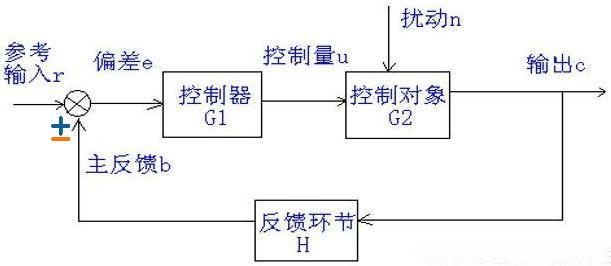
\includegraphics[width=\textwidth]{automatic control} 
\caption{自动控制系统方框图}
\end{figure}
\end{minipage}
%------------------------------------------------
\paragraph{分类}~\\
\begin{table}[H]
\centering
\begin{tabular}{|c|c|c|c|c|c|}
\hline
& 价格 & 复杂度 & 精度 & 抗干扰性能 & 其它 \\
\hline
开环 & 低 & 简单 & 低 & 差 & 稳定 \\
\hline
闭环/反馈 & 高 & 复杂 & 高 & 强 & \\
\hline
前馈 & 高 & & & & 补偿可测量扰动 \\
\hline
复合 & \multicolumn{5}{c|}{闭环 + 前馈} \\
\hline
\end{tabular}
\caption{控制方式分类}
\end{table}

\begin{minipage}[t]{0.35\textwidth}
输入量变化特性:
\begin{itemize}
\item 恒值。
\item 随动:未知时间函数。
\item 程序控制:预设时间函数。
\end{itemize}
\end{minipage}
\begin{minipage}[t]{0.35\textwidth}
系统特性:
\begin{itemize}
\item 非线性:常数、幂。
\item 线性:导数。(齐次性,线性)
\begin{itemize}
\item 定常:常系数。
\item 时变:系数不全是常数。
\item 时延:变量位移。
\end{itemize}
\end{itemize}
\end{minipage}
\begin{minipage}[t]{0.3\textwidth}
传输数据类型:
\begin{itemize}
\item 连续。
\item 离散。
\end{itemize}
\end{minipage}
%------------------------------------------------
\paragraph{性能}
\begin{itemize}
\item 稳定性:有无稳态。
\item 快速性:到达稳态快慢。
\item 准确性:稳态误差大小。
\end{itemize}
%------------------------------------------------
\paragraph{外作用}
\begin{table}[H]
\centering
\begin{tabular}{|c|c|c|c|c|c|c|}
\hline
信号 & 阶跃 & 斜坡 & 加速度 & 脉冲 & 脉动 & 正弦 \\
\hline
$ f(t)(t \geq 0) $ & $ R(t) $ & $ Rt $ & $ \frac{1}{2}R t^2 $ & $ f(0) = \infty, \int_{-\infty}^{\infty} f(t) dt = A $ & & $ A \sin(\omega t - \phi) $ \\
\hline
单位化 & \multicolumn{3}{c|}{$ R = 1 $} & $ A = 1, \delta(t) $ & & \\
\hline
图像 & 
\begin{tikzpicture}[scale=0.4] \draw[->] (0,0) -- (2,0) node[right,font=\tiny] {$ t $}; \draw[->] (0,0) -- (0,1.5) node[above,font=\tiny] {$ f(t) $}; \draw[thick] (0,0) -- (0,1) -- (2,1); \node[below,font=\tiny] at (0,0) {$ 0 $}; \node[left,font=\tiny] at (0,1) {$ R $}; \end{tikzpicture} & 
\begin{tikzpicture}[scale=0.4] \draw[->] (0,0) -- (2,0) node[right,font=\tiny] {$ t $}; \draw[->] (0,0) -- (0,2) node[above,font=\tiny] {$ f(t) $}; \draw[thick] (0,0) -- (2,2); \node[below,font=\tiny] at (0,0) {$ 0 $}; \end{tikzpicture} & 
\begin{tikzpicture}[scale=0.4] \draw[->] (0,0) -- (2,0) node[right,font=\tiny] {$ t $}; \draw[->] (0,0) -- (0,2) node[above,font=\tiny] {$ f(t) $}; \draw[thick] (0,0) parabola (2,2); \node[below,font=\tiny] at (0,0) {$ 0 $}; \end{tikzpicture} & 
\begin{tikzpicture}[scale=0.4] \draw[->] (0,0) -- (1.5,0) node[right,font=\tiny] {$ t $}; \draw[->] (0,0) -- (0,2) node[above,font=\tiny] {$ f(t) $}; \draw[thick] (0,0) -- (0,1.5); \draw[thick] (0,1.5) -- (0.1,1.5); \node[below,font=\tiny] at (0,0) {$ 0 $}; \end{tikzpicture} & 
\begin{tikzpicture}[scale=0.4] \draw[->] (0,0) -- (1.5,0) node[right,font=\tiny] {$ t $}; \draw[->] (0,0) -- (0,2) node[above,font=\tiny] {$ f(t) $}; \draw[thick] (0,1.5) -- (1,1.5); \draw[thick] (1,1.5) -- (1,0); \node[below,font=\tiny] at (0,0) {$ 0 $}; \end{tikzpicture} &  
\begin{tikzpicture}[scale=0.4] \draw[->] (0,0) -- (2.5,0) node[right,font=\tiny] {$ t $}; \draw[->] (0,0) -- (0,1.5) node[above,font=\tiny] {$ f(t) $}; \draw[thick] plot[domain=0:2,samples=50] (\x,{sin(\x r)}); \node[below,font=\tiny] at (0,0) {$ 0 $}; \end{tikzpicture} \\
\hline
\end{tabular}
\caption{典型输入信号}
\end{table}
%------------------------------------------------
\subsection[数学模型]{数学模型}
%------------------------------------------------
\subsubsection[拉氏变换]{拉氏变换}
$$ \text{微分方程(时域)}\overset{\text{拉氏变换}}{\Longrightarrow} \text{代数方程(频域)} \overset{\text{求解}}{\Longrightarrow} \text{输出量表达式(频域)} \overset{\text{反拉氏变换}}{\Longrightarrow} \text{方程解(时域)} $$
%------------------------------------------------
\paragraph{变换}
单边衰减的傅里叶变换,记$ s = \sigma + j \omega t $
$$ F(s) = L[f(t)] = \int_0^{\infty} f(t) e^{-st} dt = \int_0^{\infty} f(t) e^{-\sigma t} e^{-j \omega t} dt $$

而傅里叶变换为$ F(\omega) = \int_{-\infty}^{\infty} g(t) e^{-j \omega t} dt $。
%------------------------------------------------
\paragraph{性质}
\begin{itemize}
\item 微分定理(非零初始条件):$ L[f^{(n)}(t)] = s^n F(s) - f^{(n - 1)}(0) - s f^{(n - 2)}(0) - \dots - s^{n - 1} f(0) $。
\item 线性:$ f(t) = f_1(t) + f_2(t) \Rightarrow F(s) = F_1(s) + F_2(s) $。
\item 终值定理:$ f(\infty) = \lim_{s \to 0} sF(s) $。\\
初值定理:$ f(0^+) = \lim_{t \to 0^+} f(t)  = \lim_{s \to \infty} sF(s) $。
\item 位移定理:$ L[f(t)] = F(s) \Rightarrow L[f(t - \tau)] = e^{-\tau s}F(s), L[f(t)e^{\alpha t}] = F(s - \alpha) $。
\item 相似定理:$ L[f(t)] = F(s) \Rightarrow L[f(\frac{t}{a})] = aF(as) $。
\end{itemize}
%------------------------------------------------
\paragraph{常用变换}
\begin{table}[H]
\centering
\begin{tabular}{|c|c|c|c|c|c|c|c|c|}
\hline
时域 & $ \delta(t) $ & $ 1(t) $ & $ \frac{t^{n - 1}}{(n - 1)!} $ & $ e^{-at} $ & $ \sin \omega t $ & $ \cos \omega t $ & $ e^{-at} \sin \omega t $ & $ e^{-at} \cos \omega t $ \\
\hline
频域 & $ 1 $ & $ \frac{1}{s} $ & $ \frac{1}{s^n} $ & $ \frac{1}{s + a} $ & $ \frac{\omega}{s^2 + \omega^2} $ & $ \frac{s}{s^2 + \omega^2} $ & $ \frac{\omega}{(s + a)^2 + \omega^2} $ & $ \frac{s + a}{(s + a)^2 + \omega^2} $ \\
\hline
\end{tabular}
\caption{典型输入信号}
\end{table}
%------------------------------------------------
\subsubsection[控制微分方程]{控制微分方程}
$$ \text{输入输出方程} \Rightarrow \text{按信号传递顺序列微分方程} \Rightarrow \text{消去中间变量} \Rightarrow \text{输出量归一得到标准形式} $$
%------------------------------------------------
\paragraph{非线性微分方程的线性化}
\begin{itemize}
\item 泰勒展开:$ y = f(x_0) + \frac{d f(x)}{dx}|_{x_0} \cdot \Delta x + o(\Delta x) $。
\item 增量线性化方程:$ \Delta y = \frac{d f(x)}{dx}|_{x_0} \cdot \Delta x $。
\end{itemize}
%------------------------------------------------
\paragraph{解}
\begin{itemize}
\item 解 = 特解 + 通解(特征根)。
\item 解的模态:几点。
\end{itemize}
%------------------------------------------------
\subsubsection[传递函数]{传递函数}
%------------------------------------------------
\paragraph{概念}
系统在零初始条件下,输出输入量拉式变换之比,$ G(s) = \frac{C(s)}{R(s)} $。反应线性系统特性,与输入量无关,对应微分方程为$ s $的有理真分式。
%------------------------------------------------
\paragraph{求解}
\begin{itemize}
\item 零初始条件:$ G(s) = L[g(t)] $,其中$ g(t) $为单位脉冲响应(等效反馈函数)。
\item 非零初始条件:微分定理。
\end{itemize}
%------------------------------------------------
\paragraph{应用}
$$ R(s) = L[r(t)] \Rightarrow C(s) = G(s)R(S) \Rightarrow c(t) = L^{-1}[C(s)] $$
%------------------------------------------------
\paragraph{输入输出关系}
输入是微积分关系,则输出也是,常数用零初始条件确定。
$$ r_2(t) = \dot{r_1(t)} \Rightarrow c_2(t) = \dot{c_1(t)} $$
%------------------------------------------------
\paragraph{零极点}
\begin{align*}
G(s) &= \frac{C(s)}{R(s)} = \frac{b_0 s^m + b_1 s^{m - 1} + \dots + b_m}{a_0 s^n + a_1 s^{n - 1} + \dots + a_n}, \quad n > m \\
&= K^* \frac{\Pi_{i = 1}^m (s - z_i)}{\Pi_{j = 1}^n (s - p_j)}
\end{align*}

\begin{itemize}
\item 零点$ z_i $:影响比重、曲线形状,不决定模态。
\item 极点$ p_j $:特征根,决定模态,对系统响应影响大(近原点、远零点的影响大)。
\item 传递系数/根轨迹增益$ K^* $。
\end{itemize}
%------------------------------------------------
\paragraph{典型传递函数}
\begin{table}[H]
\centering
\begin{tabular}{|c|c|c|c|c|}
\hline
 & 微分方程 & 输出$ X_c(t) $ & 传递函数$ G(s) $ & 图像 \\
\hline
比例 & \multicolumn{2}{c|}{$ X_c(t) = KX_r(t) $} & $ K $ & 
\begin{tikzpicture}[scale=0.4] \draw[->] (0,0) -- (2,0) node[right,font=\tiny] {$ t $}; \draw[->] (0,0) -- (0,2) node[above,font=\tiny] {$ X_c(t) $}; \draw[thick] (0,0) -- (0,1.5) -- (2,1.5); \node[below,font=\tiny] at (0,0) {$ 0 $}; \node[left,font=\tiny] at (0,1.5) {$ K $}; \end{tikzpicture} \\
\hline
惯性 & $ T\frac{d X_c(t)}{dt} + X_c(t) = X_r(t) $ & $ 1 - e^{-\frac{t}{T}} $ & $ \frac{1}{Ts + 1} $ & 
\begin{tikzpicture}[scale=0.4] \draw[->] (0,0) -- (2,0) node[right,font=\tiny] {$ t $}; \draw[->] (0,0) -- (0,2) node[above,font=\tiny] {$ X_c(t) $}; \draw[thick] (0,0) plot[domain=0:2,samples=20] (\x,{1.5*(1-exp(-2*\x))}); \node[below,font=\tiny] at (0,0) {$ 0 $}; \draw[dashed,thin] (0,1.5) -- (2,1.5); \draw[dashed,thin] (0,0.948) -- (0.347,0.948); \draw[dashed,thin] (0.347,0) -- (0.347,0.948); \node[left,font=\tiny] at (0,1.5) {$ 1 $}; \node[left,font=\tiny] at (0,0.948) {$ 0.632 $}; \node[below,font=\tiny] at (0.347,0) {$ T $}; \end{tikzpicture} \\
\hline
积分 & $ X_c(t) = K \int X_r(t) dt $ & $ t $ & $ \frac{K}{s} $ & 
\begin{tikzpicture}[scale=0.4] \draw[->] (0,0) -- (2,0) node[right,font=\tiny] {$ t $}; \draw[->] (0,0) -- (0,2) node[above,font=\tiny] {$ X_c(t) $}; \draw[thick] (0,0) -- (2,2); \node[below,font=\tiny] at (0,0) {$ 0 $}; \end{tikzpicture} \\
\hline
微分 & $ X_c(t) = K \frac{d X_r(t)}{dt} $ & $ \delta(t) $ & $ Ks $ & 
\begin{tikzpicture}[scale=0.4] \draw[->] (0,0) -- (2,0) node[right,font=\tiny] {$ t $}; \draw[->] (0,0) -- (0,2) node[above,font=\tiny] {$ X_c(t) $}; \draw[thick] (0,0) -- (0,1.5); \node[below,font=\tiny] at (0,0) {$ 0 $}; \end{tikzpicture} \\
\hline
滞后 & \multicolumn{2}{c|}{$ X_c(t) = X_r(t - \tau) $} & $ e^{-Ts} $ &
\begin{tikzpicture}[scale=0.4] \draw[->] (0,0) -- (2,0) node[right,font=\tiny] {$ t $}; \draw[->] (0,0) -- (0,2) node[above,font=\tiny] {$ X_c(t) $}; \draw[thick] (0,0) -- (0.5,0) -- (0.5,1.5) -- (2,1.5); \node[below,font=\tiny] at (0,0) {$ 0 $}; \node[below,font=\tiny] at (0.5,0) {$ \tau $}; \end{tikzpicture} \\
\hline
\end{tabular}
\caption{典型传递函数(单位阶跃)}
\end{table}
%------------------------------------------------
\paragraph{开环与闭环}
\begin{itemize}
\item 开环(断开主反馈):$ G_k(s) = G(s)H(s) $。
\item 闭环:$ G_B(s) = \frac{G(s)}{1 + G_k(s)} $。
\end{itemize}
%------------------------------------------------
\subsubsection[结构图]{结构图}
\begin{figure}[H]
\centering 
\begin{tikzpicture}
\node[sum] at (0,0) {$ X $};
\node[block] at (3,0) {控制器$ G(s) $};
\node[block] at (3,-1.5) {反馈$ H(s) $};
\node at (-2,0) {输入$ R(s) $};
\node at (7.9,0) {输出$ C(s) $};
\node at (1,0.5) {偏差$ E(s) $};
\node at (1,-1.8) {反馈$ B(s) $};
\node at (6,0.5) {引出/测量点};
\node at (0,-0.7) {比较/综合点};
\draw[arrow] (4.2,0) -- (7,0);
\draw[arrow] (-1.2,0) -- (-0.4,0);
\draw[arrow] (0.4,0) -- (1.8,0);
\draw[arrow] (6,0) |- (6,-1.5) -| (4,-1.5);
\draw[arrow] (2,-1.5) -| (0,-0.4) node[near end, left] {$ \pm $};
\end{tikzpicture}
\caption{结构图}
\end{figure}
%------------------------------------------------
\paragraph{简化}
原则:等效原则,引出点信号保持不变。
\begin{itemize}
\item 串联和并联积。
\item 反馈:$ \frac{G(s)}{1 \mp G(s)H(s)} $。
\item 比较点、引出点移动:前后通路/回路乘积不变。
\item 相邻信号相加点、同一信号分支点位置可互换,二者间不可互换。
\end{itemize}
%------------------------------------------------
\subsubsection[信号流图]{信号流图}
适用于复杂系统。
%------------------------------------------------
\paragraph{概念}
\begin{figure}[H]
\centering 
\begin{tikzpicture}
\node[sum] at (0,0) {$ R $};
\node[sum] at (2,0) {$ E $};
\node[sum] at (4,0) {$ P $};
\node[sum] at (6,0) {$ Q $};
\node[sum] at (8,0) {$ C $};
\node at (4,-0.8) {$ -H $};
\node at (0,-0.7) {输入节点/源点};
\node at (8,-0.7) {输出节点/阱点};
\node at (4,0.7) {混合节点};
\node at (1,0.7) {支路};
\draw[arrow] (0.4,0) -- (1.6,0) node[midway, above] {$ 1 $};
\draw[arrow] (2.4,0) -- (3.6,0) node[midway, above] {$ G_1 $};
\draw[arrow] (4.4,0) -- (5.6,0) node[midway, above] {$ G_2 $};
\draw[arrow] (6.4,0) -- (7.6,0) node[midway, above] {$ 1 $};
\draw[arrow] (5.7,-0.2) to[bend left=60] (2.3,-0.2);
\end{tikzpicture}
\caption{信号流图}
\end{figure}

\begin{itemize}
\item 混合节点:流向该结点信号代数和。
\item 支路:方向 + 传递函数,相当于乘法器,保证信号单向传递。
\item 前向通路:输入到输出,不重复过节点。
\item 回路:起止于同一节点,不重复过节点。
\item 不接触回路:回路间无公共节点。
\end{itemize}
%------------------------------------------------
\paragraph{简化}
\begin{itemize}
\item 串联积并联和。
\item 回路消除:反馈消去。\\
自回路消除:节点自延长,增益为$ 1 $,有回路,反馈消去。
\end{itemize}
%------------------------------------------------
\paragraph{绘制}
根据结构图或拉屎变换得到的微分方程。
\begin{itemize}
\item 节点:比较点右侧、分支点,可多画再删除。
\item 源点、阱点不要和相邻节点合并。
\end{itemize}
%------------------------------------------------
\paragraph{梅森公式}
\begin{align*}
P &= \frac{1}{\underbrace{\Delta}_{\text{简单回路}}} \sum_{k = 1}^n \underbrace{P_k}_{\text{前向通路}} \Delta_k \\
\Delta &= 1 - \sum_{L_i} + \sum_{L_i, L_j} - \sum_{L_i, L_j, L_r} + \dots
\end{align*}

其中,$ \Delta_k $是余子式,由$ \Delta $略去与$ P_k $接触项获得。
\begin{itemize}
\item 两节点间增益为$ 1 $,若合并后两回路接触,则不可合并。
\item 求解的是输出对输入的增益,若求解中间变量,可省去前面输入、比值进行计算。
\end{itemize}
%----------------------------------------------------------------------------------------
\section{时域分析}
%------------------------------------------------
\subsection[性能指标]{性能指标}
典型输入信号:线性系统选取单位阶跃信号。

\begin{figure}[H]
\centering 
\begin{tikzpicture}[scale=1]
\draw[->] (0,0) -- (8,0) node[right] {$ t $};
\draw[->] (0,0) -- (0,3) node[above] {$ h(t) $};
\draw[dashed, gray] (0,2) -- (8,2);
\draw[dashed, gray, very thin] (0,1.9) -- (8,1.9);
\draw[dashed, gray, very thin] (0,2.1) -- (8,2.1);
\node at (7,2.5) {误差带};
\draw[thick, blue] plot[domain=0:7.5, samples=100] (\x, {2*(1 - exp(-0.3*\x)*cos(deg(1.2*\x)))});
\node[below] at (0,0) {$ 0 $};
\node[left] at (0,2) {$ 1 $};
\coordinate (peak) at (2.618,2.91);
\draw[dotted] (peak) -- (2.618,0) node[below] {$ t_p $};
\draw[dotted] (peak) -- (0,2.91) node[left] {$ h(t_p) $};
\draw[dotted] (6.2,0) -- (6.2,2);
\node[below] at (6.2,0) {$ t_s $};
\draw[dotted] (1.309,2) -- (1.309,0) node[below] {$ t_r $};
\draw[<->, thick, red] (0,-0.6) -- (6.2,-0.6);
\node[below, red] at (3.1,-0.6) {动态过程响应过程};
\node[below] at (3.1,-1.1) {响应过程};
\draw[<->, thick, green] (6.2,-0.6) -- (7.5,-0.6);
\node[below, green] at (6.85,-0.6) {稳态过程};
\node[below] at (6.85,-1.1) {输出复现输入的程度};
\node[below] at (4,1) {跟踪误差$ e(t) = r(t) - c(t) $};
\end{tikzpicture}
\caption{二阶欠阻尼系统}
\end{figure}

\begin{table}[H]
\centering
\begin{tabular}{|c|c|c|c|}
\hline
状态 & 指标 & 符号 & 定义 \\
\hline
\multirow{5}{*}{动态} & 延迟时间 & $ t_d $ & 首次达到终值$ 50\% $的时间 \\
\cline{2-4}
& 上升时间 & $ t_r $ & 终值$ 10\% - 90\% $的时间(有振荡系统为$ 0\% - 100\% $) \\
\cline{2-4}
& 峰值时间 & $ t_p $ & 首次达到最大值的时间 \\
\cline{2-4}
& 超调量 & $ \sigma $ & $ \frac{h(t_p) - h(\infty)}{h(\infty)} \times 100\% $ \\
\cline{2-4}
& 调整时间 & $ t_s $ & 达到并保持在误差带的时间 \\
\hline
稳态 & 稳态误差 & $ ess $ & $ e(t)|_{t \to \infty} = r(t)|_{t \to \infty} - h(t)|_{t \to \infty} $ \\
\hline
\end{tabular}
\caption{性能指标}
\end{table}
%------------------------------------------------
\subsection[一阶系统]{一阶系统}
\begin{figure}[H]
\centering 
\begin{tikzpicture}
\node[sum] at (0,0) {$ X $};
\node[block] at (3,0) {$ \frac{1}{Ts} $};
\node at (-1.6,0) {$ R(s) $};
\node at (7.5,0) {$ C(s) $};
\node at (1,0.2) {$ E(s) $};
\node at (5.5,0.4) {$ \Phi(s) = \frac{1}{1 + Ts} $};
\draw[arrow] (4,0) -- (7,0);
\draw[arrow] (-1.2,0) -- (-0.4,0);
\draw[arrow] (0.4,0) -- (2,0);
\draw[arrow] (6,0) |- (6,-1) -| (0,-0.4) node[near end, left] {$ - $};
\end{tikzpicture}
\caption{一阶系统结构图}
\end{figure}
%------------------------------------------------
\paragraph{响应情况}
\begin{table}[H]
\centering
\begin{tabular}{|c|c|c|c|c|c|}
\hline
$ r(t) \to R(s) $ & $ c(t) $ & $ e(t) $ & $ e_{ss} $ & 备注 & 图像 \\
\hline
$ 1(t) \to \frac{1}{s} $ & $ 1 - e^{-\frac{t}{T}} $ & $ -\frac{1}{T}e^{-\frac{t}{T}} $ & $ 0 $ & &
\begin{tikzpicture}[scale=0.4] \draw[->] (0,0) -- (2,0) node[right,font=\tiny] {$ t $}; \draw[->] (0,0) -- (0,1.5) node[above,font=\tiny] {$ h(t) $}; \draw[thick] (0,0) plot[domain=0:2,samples=20] (\x,{1.2*(1-exp(-2*\x))}); \draw[dashed,thin] (0,1.2) -- (2,1.2); \node[below,font=\tiny] at (0,0) {$ 0 $}; \node[left,font=\tiny] at (0,1.2) {$ 1 $}; \end{tikzpicture} \\
\hline
$ \delta(t) \to 1 $ & $ \frac{1}{T} e^{-\frac{t}{T}} $ & $ -\frac{1}{T}e^{-\frac{t}{T}} $ & $ 0 $ & & 
\begin{tikzpicture}[scale=0.4] \draw[->] (0,0) -- (2,0) node[right,font=\tiny] {$ t $}; \draw[->] (0,0) -- (0,1.5) node[above,font=\tiny] {$ h(t) $}; \draw[thick] (0,1.2) plot[domain=0:2,samples=20] (\x,{1.2*exp(-2*\x)}); \node[below,font=\tiny] at (0,0) {$ 0 $}; \node[left,font=\tiny] at (0,1.2) {$ \frac{1}{T} $}; \end{tikzpicture} \\
\hline
$ t \to \frac{1}{s^2} $ & $ t - T + T e^{-\frac{t}{T}} $ & $ T(1 - e^{-\frac{t}{T}}) $ & $ T $ & $ T $越小跟踪精度越高 & 
\begin{tikzpicture}[scale=0.4] \draw[->] (0,0) -- (2,0) node[right,font=\tiny] {$ t $}; \draw[->] (0,0) -- (0,1.5) node[above,font=\tiny] {$ h(t) $}; \draw[thick] (0,0) plot[domain=0:2,samples=20] (\x,{\x-0.5+0.5*exp(-2*\x)}); \draw[dashed,thin] (0,0) -- (2,2); \node[below,font=\tiny] at (0,0) {$ 0 $}; \end{tikzpicture} \\
\hline
$ \frac{1}{2}t^2 \to \frac{1}{s^3} $ & $ (\frac{1}{2}t^2 + Tt) + T^2(1 - e^{-\frac{t}{T}}) $ & $ Tt - T^2(1 - e^{-\frac{t}{T}}) $ & $ \infty $ & 无法跟踪 & \\
\hline
\end{tabular}
\caption{一阶系统响应情况}
\end{table}
%------------------------------------------------
\paragraph{单位阶跃响应}
$ T $越大,惯性越大,响应越慢。
\begin{align*}
h(T) &= 0.632,& \quad h(2T) &= 0.865,& \quad h(3T) &= 0.95 \\
t_d &= 0.69T,& \quad t_r &= 2.2T,& \quad t_s &= 3T
\end{align*}
%------------------------------------------------
\subsection[二阶系统]{二阶系统}
\begin{figure}[H]
\centering 
\begin{tikzpicture}
\node[sum] at (0,0) {$ X $};
\node[block] at (3,0) {$ \frac{\omega_n^2}{s(s + 2 \xi \omega_n)} $};
\node at (-1.6,0) {$ R(s) $};
\node at (7.5,0) {$ C(s) $};
\node at (1,0.2) {$ E(s) $};
\node at (4,1) {$ \Phi(s) = \frac{\omega_n^2}{s^2 + 2 \xi \omega_n s + \omega_n^2} $};
\draw[arrow] (4,0) -- (7,0);
\draw[arrow] (-1.2,0) -- (-0.4,0);
\draw[arrow] (0.4,0) -- (2,0);
\draw[arrow] (6,0) |- (6,-1) -| (0,-0.4) node[near end, left] {$ - $};
\end{tikzpicture}
\caption{二阶系统结构图}
\end{figure}
%------------------------------------------------
\paragraph{概念}
\begin{itemize}
\item 自然角频率(无阻尼振荡圆频率)$ \omega_n > 0 $。
\item 阻尼比$ \xi $:增大过程中,从无衰减周期运动变为有衰减正弦运动,最后无振荡。$ \xi > 1 $,$ t_s $长;$ \xi \leq 0 $,不能稳定工作;$ \xi $较小时,$ \sigma $大,振荡次数多,$ t_s $长;最佳为$ \xi = \frac{1}{\sqrt{2}} \approx 0.707 $。
\item 特征方程$ s^2 + 2 \xi \omega_n s + \omega_n^2 $。
\item 特征根($ 0 < \xi < 1 $):
$$ s_{1, 2} = -\underbrace{\xi \omega_n}_{\text{衰减系数}\sigma} \pm j \underbrace{\omega_n \sqrt{1 - \xi^2}}_{\text{阻尼振荡圆频率}\omega_d} $$
阻尼角$ \beta = \arctan(\frac{\omega_d}{\sigma}) $。
\item 特征根($ \xi > 1 $):
$$ s_{1, 2} = -\xi \omega_n \pm \omega_n \sqrt{\xi^2 - 1} $$
以$ T_{1, 2} = \frac{1}{\omega_n(\xi \pm \sqrt{\xi^2 - 1})} $,则$ s_{1, 2} = -\frac{1}{T_{1, 2}}, s_1 s_2 = \frac{1}{T_1 T_2} = \omega_n^2 $。
\end{itemize}
%------------------------------------------------
\paragraph{阻尼情况讨论}
\begin{table}[H]
\centering
\begin{tabular}{|c|c|c|c|c|c|}
\hline
$ \xi $ & 阻尼 & 阶跃响应 & 稳定性 & $ C(s) $ & $ c(t) $ \\
\hline
$ (-\infty, 0) $ & 负 & 振荡/发散 & 不稳定 & & \\
\hline
$ 0 $ & 无/零 & 等幅振荡 & 临界 & $ \frac{1}{s} - \frac{s}{s^2 + \omega_n^2} $ & $ 1 - \cos \omega_n t $ \\
\hline
$ (0, 1) $ & 欠 & 衰减振荡 & 稳定 & $ \frac{1}{s} - \frac{s + 2\xi \omega_n}{s^2 + 2 \xi \omega_n s + \omega_n^2} $ & $ 1 - \frac{e^{-\sigma t}}{\sqrt{1 - \xi^2}}\sin(\omega_d t + \beta) $ \\
\hline
$ 1 $ & 临界 & 单升非振荡 & 稳定 & $ \frac{1}{s} - \frac{1}{s + \omega_n} - \frac{\omega_n}{(s + \omega_n)^2} $ & $ 1 - e^{-\omega_n t}(1 + \omega_n t) $ \\
\hline
$ (1, \infty) $ & 过 & 单升非振荡 & 稳定 & $ \frac{1}{s} + \frac{T_1}{T_2 - T_1}\frac{1}{s + \frac{1}{T_1}} + \frac{T_2}{T_1 - T_2}\frac{1}{s + \frac{1}{T_2}} $ & $ 1 + \frac{T_1}{T_2 - T_1} e^{-\frac{t}{T_1}}+ \frac{T_2}{T_1 - T_2} e^{-\frac{t}{T_2}} $ \\
\hline
\end{tabular}
\caption{阻尼情况讨论}
\end{table}
%------------------------------------------------
\paragraph{动态性能}
\begin{itemize}
\item $ 0 < \xi < 1 $:
\begin{itemize}
\item $ t_d = \frac{1 + 0.7\xi}{\omega_n} $。
\item $ t_r(0 - 100\%) = \frac{\pi - \beta}{\omega_d} $。
\item $ t_p = \frac{\pi}{\omega_d} $。
\item $ \sigma = e^{-\frac{\xi \pi}{\sqrt{1 - \xi^2}}} \times 100\% $。
\item $ t_s = -\frac{ln(\sqrt{1 - \xi^2} \times \Delta\%)}{\xi \omega_n} \Rightarrow \begin{cases} \frac{4}{\xi \omega_n}, \Delta = 2 \\  \frac{3}{\xi \omega_n}, \Delta = 5 \end{cases} $。
\end{itemize}
\item $ \xi > 1 $:
\begin{itemize}
\item $ t_d = \frac{1 + 0.6\xi + 0.2\xi^2}{\omega_n} $。
\item $ t_r(10\% - 90\%) = \frac{1 + 1.5\xi + \xi^2}{\omega_n} $。
\item $ t_s = 3T_1 $。
\end{itemize}
\item $ \xi = 1 $:$ t_s = 4.75 T_1 $,为最小值。
\item $ \xi \gg 1 $:可近似为一阶系统。
\end{itemize}
%------------------------------------------------
\paragraph{有零点的二阶欠阻尼系统}
$ \Phi(s) = \frac{\omega_n^2(1 + \tau s)}{s^2 + 2\xi \omega_n s + \omega_n^2} $,具有零点$ z = \frac{1}{\tau} $。
\begin{align*}
C(s) &= \underbrace{\frac{\omega_n^2}{s^2 + 2\xi \omega_n s + \omega_n^2} \frac{1}{s}}_{c_1(s)} + \underbrace{\frac{\omega_n^2 \tau}{s^2 + 2\xi \omega_n s + \omega_n^2}}_{c_2(s)} \\
c(t) &= c_1(t) + \frac{1}{z} \frac{d c_1(t)}{dt} = 1 - \frac{e^{-\xi \omega_n t}}{\sqrt{1 - \xi^2}} \cdot \frac{l}{z} \sin(\sqrt{1 - \xi^2}\omega_n t + \beta + \varphi)
\end{align*}

其中,$ \beta = \arctan(\frac{\sqrt{1 - \xi^2}}{\xi}), \varphi = \arctan(\frac{\omega_n \sqrt{1 - \xi^2}}{z - \xi \omega_n}), l = \sqrt{z^2 - 2\xi \omega_n z + \omega_n^2} $。
%------------------------------------------------
\paragraph{改善}
\begin{figure}[H]
\centering 
\begin{tikzpicture}
\node[sum] at (0,0) {$ X $};
\node[sum] at (2.5,0) {$ X $};
\node[block] at (4.5,0) {$ \frac{\omega_n^2}{s(s + 2 \xi \omega_n)} $};
\node[block, minimum width=1cm, minimum height=0.5cm] at (1.3,1) {$ \tau s $};
\node at (-1.6,0) {$ R(s) $};
\node at (7.5,0) {$ C(s) $};
\draw[arrow] (5.5,0) -- (7,0);
\draw[arrow] (-1.2,0) -- (-0.4,0);
\draw[arrow] (0.4,0) -- (2.1,0);
\draw[arrow] (2.9,0) -- (3.5,0);
\draw[arrow] (6,0) |- (6,-0.8) -| (0,-0.4) node[near end, left] {$ - $};
\draw[arrow] (0.5,0) |- (0.5,1) -| (0.8,1);
\draw[arrow] (1.8,1) |- (2.5,1) -| (2.5,0.4) node[near end, right] {$ + $};
\end{tikzpicture}
\begin{tikzpicture}
\node[sum] at (0,0) {$ X $};
\node[sum] at (1.5,0) {$ X $};
\node[block] at (4.5,0) {$ \frac{\omega_n^2}{s(s + 2 \xi \omega_n)} $};
\node[block, minimum width=1cm, minimum height=0.5cm] at (3,-0.8) {$ \tau s $};
\node at (-1.6,0) {$ R(s) $};
\node at (7.5,0) {$ C(s) $};
\draw[arrow] (5.5,0) -- (7,0);
\draw[arrow] (-1.2,0) -- (-0.4,0);
\draw[arrow] (0.4,0) -- (1.1,0);
\draw[arrow] (1.9,0) -- (3.5,0);
\draw[arrow] (6,-0.8) -- (3.5,-0.8);
\draw[arrow] (6,0) |- (6,-1.2) -| (0,-0.4) node[near end, left] {$ - $};
\draw[arrow] (2.5,-0.8) |- (1.5,-0.8) -| (1.5,-0.4) node[near end, left] {$ - $};
\end{tikzpicture}
\caption{改善二阶系统结构图}
\end{figure}

\begin{itemize}
\item PD(微分顺馈):$ \omega_n $不变,$ \xi_d = \xi + \frac{\tau}{2} \omega_m $,零点$ z = -\frac{1}{\tau} $,放大噪声。
\item 测速反馈:$ \omega_n $不变,$ \xi_t = \xi + \frac{\tau}{2} \omega_m $。
\end{itemize}
%------------------------------------------------
\subsection[稳定性分析]{稳定性分析}
%------------------------------------------------
\paragraph{概念}
$$ G_B(s) = \frac{b_0 s^m + b_1 s^{m - 1} + \dots + b_m}{a_0 s^n + a_1 s^{n - 1} + \dots + a_n} $$
\begin{itemize}
\item 稳定:$ t:0 \to \infty $,系统能达到新的稳态。
\item 充要条件:特征方程的根均在根平面的左半平面(闭环传递函数的极点严格分布在$ s $平面左半平面)。
\item 最小相位系统:闭环传递函数的零极点都分布在$ s $平面左半平面,必要条件为特征多项式的系数全同号(非零)。
\end{itemize}
%------------------------------------------------
\subsubsection[判据]{判据}
%------------------------------------------------
\paragraph{赫尔维茨判据}
系统稳定$ \Leftrightarrow $$ n $阶赫尔维茨矩阵$ \Delta_i > 0 $。
$$ \Delta_x = \begin{vmatrix} a_1 & a_3 & a_5 & \cdots & a_{2n - 1} \\ a_0 & a_2 & a_4 & \cdots & a_{2n - 2} \\ 0   & a_1 & a_3 & \cdots & a_{2n - 3} \\ \vdots & \vdots & \vdots & \ddots & \vdots \\ 0 & 0 & 0 & \cdots & a_n \end{vmatrix} $$

其中横向相邻项差$ 2 $,纵向相邻项差$ -1 $,对角线相邻项差$ 1 $,序数大于$ n $的项为$ 0 $。
\begin{itemize}
\item 一阶:$ a_0, a_1 > 0 $。
\item 二阶:$ a_0, a_1, a_2 > 0 $。
\item 三阶:$ a_0, a_1, a_2, a_3 > 0, a_1 a_2 - a_0 a_3 > 0 $。
\item 四阶:$ a_0, a_1, a_2, a_3, a_4 > 0, a_1 a_2 a_3 - a_1^2 a_4 - a_0 a_3^2  > 0 $。
\end{itemize}
%------------------------------------------------
\paragraph{劳斯判据}
\begin{align*}
&\begin{array}{cccccc}
s^n & a_0 & a_2 & a_4 & a_6 & \cdots \text{偶数项} \\
s^{n - 1} & a_1 & a_3 & a_5 & a_7 & \cdots \text{奇数项} \\
s^{n - 2} & b_1 & b_2 & b_3 & b_4 & \cdots \\
s^{n - 3} & c_1 & c_2 & c_3 & c_4 & \cdots \\
\vdots & \vdots & \vdots & \vdots & \vdots & \\
s^2 & e_1 & e_2 \\
s^1 & f_1 \\
s^0 & g_1 \\
\end{array} \\
& \text{其中} z_n = \frac{y_1 x_{n + 1} - x_1 y_{n + 1}}{y_1}
\end{align*}

第$ i $行第$ j $列的元素为$ i - 1, i - 2 $两行$ 1, j + 1 $两列的行列式的相反数比上第$ i - 1 $行第$ 1 $列的元素。
\begin{itemize}
\item 第一列元素变号次数为右半平面根数,全同号则稳定。
\item 第一列有$ 0 $,用$ \epsilon \to 0 $代替。
\item 某行全为$ 0 $,用上一行作为辅助方程(系统不稳定,判断根的情况)求导:
$$ \begin{array}{ccccc} s^n & a & b & c & \cdots \\ s^{n - 1} & na & (n - 2)b & (n - 4)c & \cdots \end{array} $$
\item 应用:求解使系统稳定的$ k $。拓展为使跟在$ -x $左侧(预留波动空间)时,用$ s = s' - x $代换,对$ s' $求解劳斯判据。
\end{itemize}
%------------------------------------------------
\subsubsection[稳态误差]{稳态误差}
$ c(t) $ = 稳态 + 暂态($ t \to \infty $,稳定系统暂态$ \to 0 $)。
\begin{figure}[H]
\centering 
\begin{tikzpicture}
\node[sum] at (0,0) {$ X $};
\node[block] at (3,0) {$ G(s) $};
\node[block] at (3,-1.5) {$ H(s) $};
\node at (-1,0.3) {$ R(s) $};
\node at (-1,-0.3) {$ r(t) $};
\node at (1,0.3) {$ E(s) $};
\node at (1,-0.3) {$ e(t) $};
\node at (6.5,0.3) {$ C(s) $};
\node at (6.9,-0.3) {实际$ c(t) $};
\node at (7,-0.9) {期望$ c_d(t) $};
\node at (1,-1.2) {$ B(s) $};
\node at (1,-1.8) {$ b(t) $};
\draw[arrow] (4,0) -- (7,0);
\draw[arrow] (-1.2,0) -- (-0.4,0);
\draw[arrow] (0.4,0) -- (2,0);
\draw[arrow] (6,0) |- (6,-1.5) -| (4,-1.5);
\draw[arrow] (2,-1.5) -| (0,-0.4) node[near end, left] {$ - $};
\end{tikzpicture}
\caption{稳态误差}
\end{figure}
%------------------------------------------------
\paragraph{误差}
\begin{itemize}
\item 给定误差(输入端)$ E(s) $:
\begin{align*}
&e(t) = r(t) - b(t) \\
\Rightarrow 
&E(s) = R(s) - B(s) = R(s) - H(s) C(s) = \frac{R(s)}{1 + G_k(s)} \\
\Rightarrow 
&ess = \lim_{s \to 0} s \cdot E(s) = \lim_{s \to 0} \frac{s R(s)}{1 + G_k(s)}
\end{align*}
\item 扰动误差(输出端)$ B(s) = E(s) - C(s) H(s) $:
\begin{align*}
&e_N(t) = c_d(t) - c(t) \\
\Rightarrow 
&E_N(s) = C_d(s) - C(s) = \frac{E(s)}{H(s)} = -C_N(s) \\
\Rightarrow 
&ess_N = \lim_{s \to 0} s \cdot E_N(s) = -\lim_{s \to 0} s \cdot C_N(s)
\end{align*}
\end{itemize}
%------------------------------------------------
\paragraph{系统类型}
$ G_k(s) = \frac{k \Pi_{i = 1}^m (\tau_i s + 1)}{s^v \Pi_{i = 1}^{n - v} (T_j s + 1)} $。

\begin{table}[H]
\centering
\begin{tabular}{|c|c|c|c|c|c|}
\hline
$ r(t) $ & $ k $ & $ ess $ & 0型 & 1型 & 2型 \\
\hline
$ 1(t) $ & $ k_p = \lim_{s \to 0} G_k(s) $ & $ \frac{1}{1 + k_p} $ & $ \frac{1}{1 + k_k} $ & $ 0 $ & $ 0 $ \\
\hline
$ t $ & $ k_v = \lim_{s \to 0} s G_k(s) $ & $ \frac{1}{k_v} $ & $ \infty $ & $ \frac{1}{k_k} $ & $ 0 $ \\
\hline
$ \frac{t^2}{2} $ & $ k_a = \lim_{s \to 0} s^2 G_k(s) $ & $ \frac{1}{k_a} $ & $ \infty $ & $ \infty $ & $ \frac{1}{k_k} $ \\
\hline
\end{tabular}
\caption{阻尼情况讨论}
\end{table}
%------------------------------------------------
\paragraph{减小稳态误差的方法}
\begin{itemize}
\item 增大开环放大系数$ k_k $:增益裕度变小,易使系统不稳定。
\item 增多积分环节$ v $:相位裕度变小,易使系统不稳定。
\item 串级控制已知内回路扰动。
\item 加前馈:
\begin{itemize}
\item 补偿给定量:$ G_c(s) = \frac{1}{G_2(s)} \Rightarrow E(s) = 0 $。
\item 补偿扰动量:$ G_c(s) = \frac{1}{G_1(s)} \Rightarrow C_N(s) = 0 $。
\end{itemize}
\end{itemize}

\begin{figure}[H]
\centering 
\begin{tikzpicture}
\node[sum] at (0,0) {$ X $};
\node[block] at (2.5,0) {$ G_1(s) $};
\node[sum] at (5,0) {$ X $};
\node[block] at (7.5,0) {$ G_2(s) $};
\node[block] at (2.5,-1.5) {$ G_c(s) $};
\node at (-2,0) {$ R(s) $};
\node at (10,0) {$ C(s) $};
\node at (1,-0.5) {$ E(s) $};
\draw[arrow] (-1.5,0) -- (-0.4,0);
\draw[arrow] (0.4,0) -- (1.5,0);
\draw[arrow] (3.5,0) -- (4.6,0);
\draw[arrow] (5.4,0) -- (6.5,0);
\draw[arrow] (8.5,0) -- (9.5,0);
\draw[arrow] (9,0) |- (9,1) -| (0,0.4) node[near end, left] {$ - $};
\draw[arrow] (-1,0) |- (-1,-1.5) -| (1.5,-1.5);
\draw[arrow] (3.5,-1.5) |- (5,-1.5) -| (5,-0.4);
\end{tikzpicture}
\begin{tikzpicture}
\node[sum] at (0,0) {$ X $};
\node[block] at (2.5,0) {$ G_1(s) $};
\node[sum] at (5,0) {$ X $};
\node[block] at (7.5,0) {$ G_2(s) $};
\node[block] at (2.5,1.5) {$ G_c(s) $};
\node at (-2,0) {$ R(s) $};
\node at (10,0) {$ C(s) $};
\node at (5.5,1.5) {$ N(s) $};
\draw[arrow] (-1.5,0) -- (-0.4,0);
\draw[arrow] (0.4,0) -- (1.5,0);
\draw[arrow] (3.5,0) -- (4.6,0);
\draw[arrow] (5.4,0) -- (6.5,0);
\draw[arrow] (8.5,0) -- (9.5,0);
\draw[arrow] (5,2) -- (5,0.4) node[near end, right] {$ + $};
\draw[arrow] (5,1.5) -- (3.5,1.5);
\draw[arrow] (1.5,1.5) |- (0,1.5) -| (0,0.4);
\draw[arrow] (9,0) |- (9,-1) |- (0,-1) -| (0,-0.4);
\end{tikzpicture}
\caption{前馈复合控制}
\end{figure}
%----------------------------------------------------------------------------------------
\section{根轨迹分析}
%------------------------------------------------
\subsection[概念]{概念}
%------------------------------------------------
\subsection[绘制]{绘制}
%------------------------------------------------
\subsection[广义根轨迹]{广义根轨迹}
%----------------------------------------------------------------------------------------
\section{频域分析}
%------------------------------------------------
\subsection[概念]{概念}
%------------------------------------------------
\subsection[图像]{图像}
%------------------------------------------------
\subsection[稳定性分析]{稳定性分析}
%----------------------------------------------------------------------------------------
\section{校正}
%------------------------------------------------
\subsection[概念]{概念}
%------------------------------------------------
\subsection[串联校正]{串联校正}
%------------------------------------------------
\subsection[反馈校正]{反馈校正}
%----------------------------------------------------------------------------------------
\section{离散系统}
%------------------------------------------------
\subsection[概念]{概念}
%------------------------------------------------
\subsection[z变换]{z变换}
%------------------------------------------------
\subsection[线性定常离散系统]{线性定常离散系统}
%----------------------------------------------------------------------------------------
\part{现代控制}
%----------------------------------------------------------------------------------------
\section{控制系统}
%------------------------------------------------
\subsection[状态空间]{状态空间}
%------------------------------------------------
\subsection[线性控制系统]{线性控制(LTI)系统}
%----------------------------------------------------------------------------------------
\section{控制系统的结构性质}
%------------------------------------------------
\subsection[能控性与能观测性]{能控性与能观测性}
%------------------------------------------------
\subsection[稳定性]{稳定性}
%----------------------------------------------------------------------------------------
\section{反馈控制系统}
%------------------------------------------------
\subsection[反馈]{反馈}
%------------------------------------------------
\subsection[李雅普诺夫方法设计反馈系统]{李雅普诺夫方法设计反馈系统}
%------------------------------------------------
\subsection[极点配置]{极点配置}
%------------------------------------------------
\subsection[解耦]{解耦}
%----------------------------------------------------------------------------------------
\section{状态观测器与动态反馈}
%------------------------------------------------
\subsection[观测器]{观测器}
%------------------------------------------------
\subsection[动态反馈]{动态反馈}
%------------------------------------------------
\subsection[鲁棒控制]{鲁棒控制}
%----------------------------------------------------------------------------------------
\part{最优控制}
%----------------------------------------------------------------------------------------
\section{最优控制}
%------------------------------------------------
\subsection[概念]{概念}
%------------------------------------------------
\subsection[各方法的关系]{各方法的关系}
%----------------------------------------------------------------------------------------
\section{连续时间最优控制}
%------------------------------------------------
\subsection[变分法]{变分法}
%------------------------------------------------
\subsection[最大值原理]{最大值原理}
%------------------------------------------------
\subsection[线性二次型]{线性二次型}
%------------------------------------------------
\subsection[动态规划]{动态规划}
%----------------------------------------------------------------------------------------
\section{离散时间最优控制}
%------------------------------------------------
\subsection[最大值原理]{最大值原理}
%------------------------------------------------
\subsection[线性二次型]{线性二次型}
%------------------------------------------------
\subsection[动态规划]{动态规划}
%----------------------------------------------------------------------------------------
\end{document}